\section{Performance}

The response of the LTCC to electrons and pions has been studied using experimental data from the spring 2019 period,
the first time that the LTCC sectors 3 and 5 were filled with the $C_4F_{10}$ gas.
At the time of this writing the data is not yet calibrated.

\subsection{LTCC Response to electrons}\label{sec:elecResponse}

The electrons are selected using the reconstruction algorithms \cite{recon-nim} that identifies electron tracks.
The LTCC response is calculated by checking whether the electrons produced a signal in the detector or not.
The electron momenta has been selected in the pion expected response range, between 3.5 and 8 GeV.
The criterias for the event selections are:

\begin{itemize}
	\item  Electrons identified using the reconstruction event builder algorithm;
    \item Electrons must be within a detector fiducial cut, see \F{electronDetFiducialCut}.
\end{itemize}

\begin{figure}
	\centering
	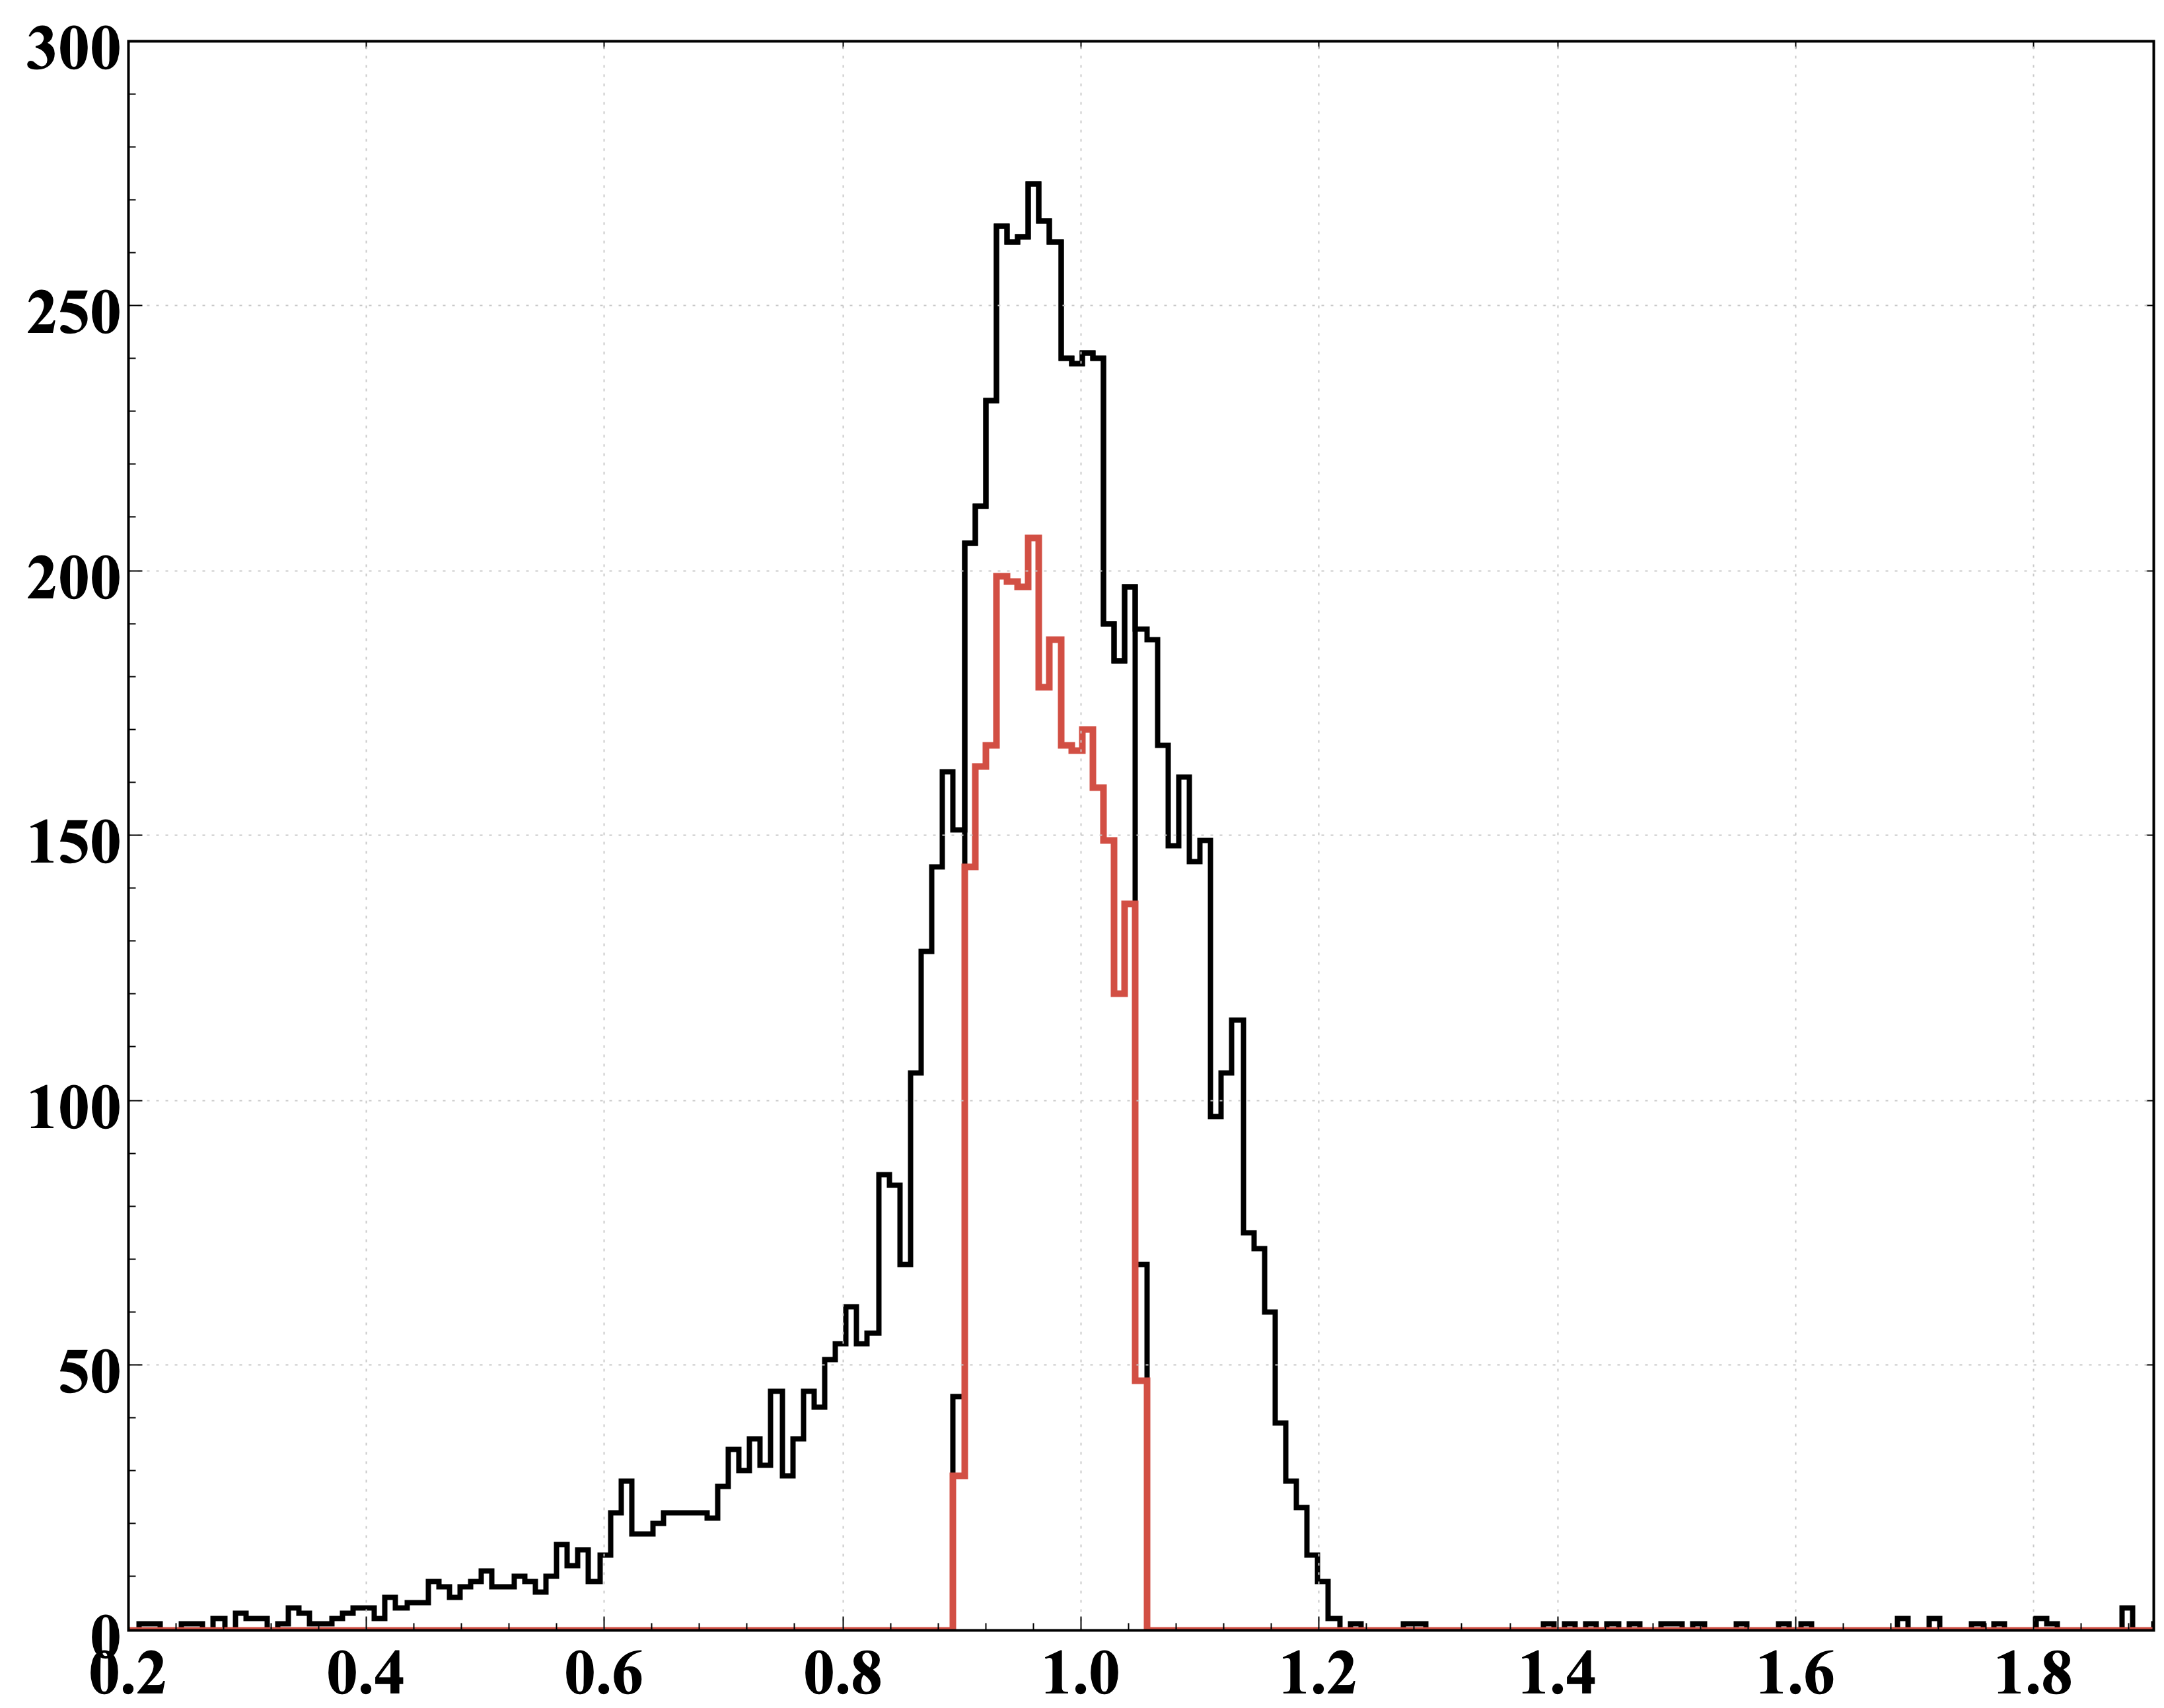
\includegraphics[width=0.98\columnwidth,keepaspectratio]{img/electronDetFiducialCut.png}
	\caption{(placeholder) The electron fiducial cut applied to electrons}
	\label{fig:electronDetFiducialCut}
\end{figure}

The electron momentum spectrum before and after the requirement of an associated LTCC signal is shown in \F{electronEfficiency},
along with a zero-order polynomial fit. The average efficiency of electrons is 94$\%$, below the expected 99$\%$.
This may be due to the fact that the electron selection did not involve the calorimeters (due to the uncalibrated detector status)
and/or by unrelated inefficiencies in other detector systems.

\begin{figure}
	\centering
	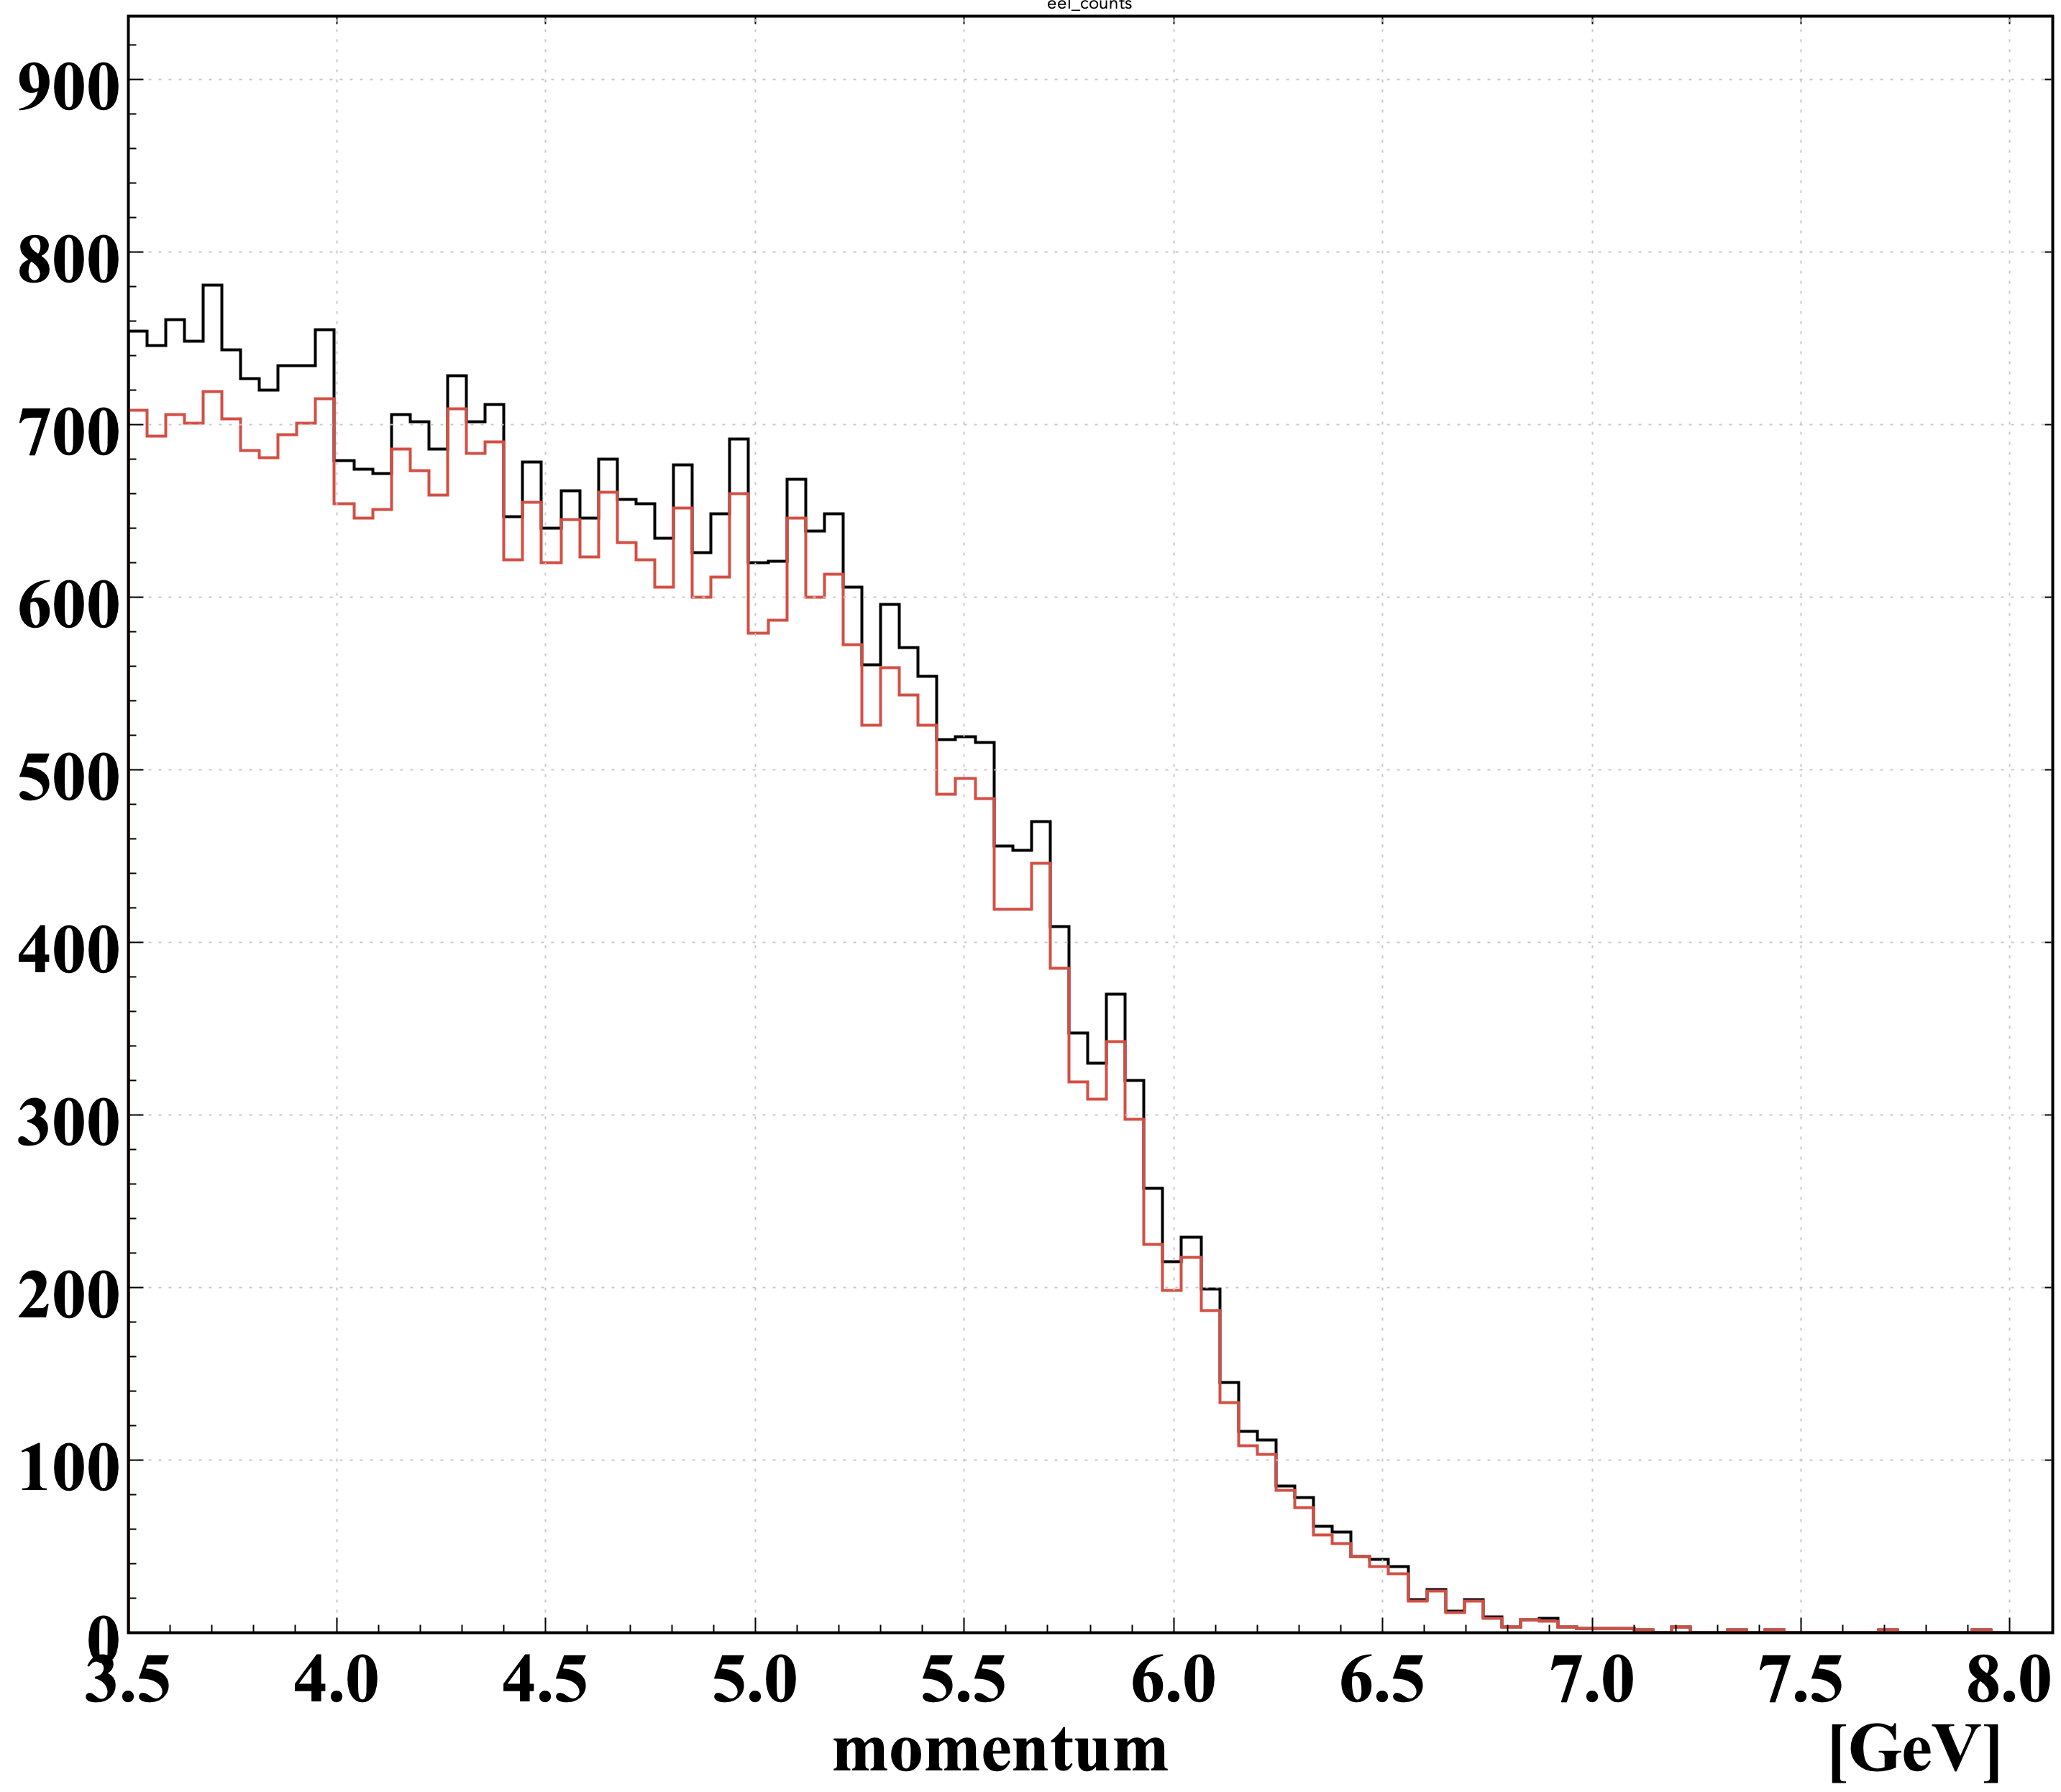
\includegraphics[width=0.98\columnwidth,keepaspectratio]{img/electronMomenta.png}
	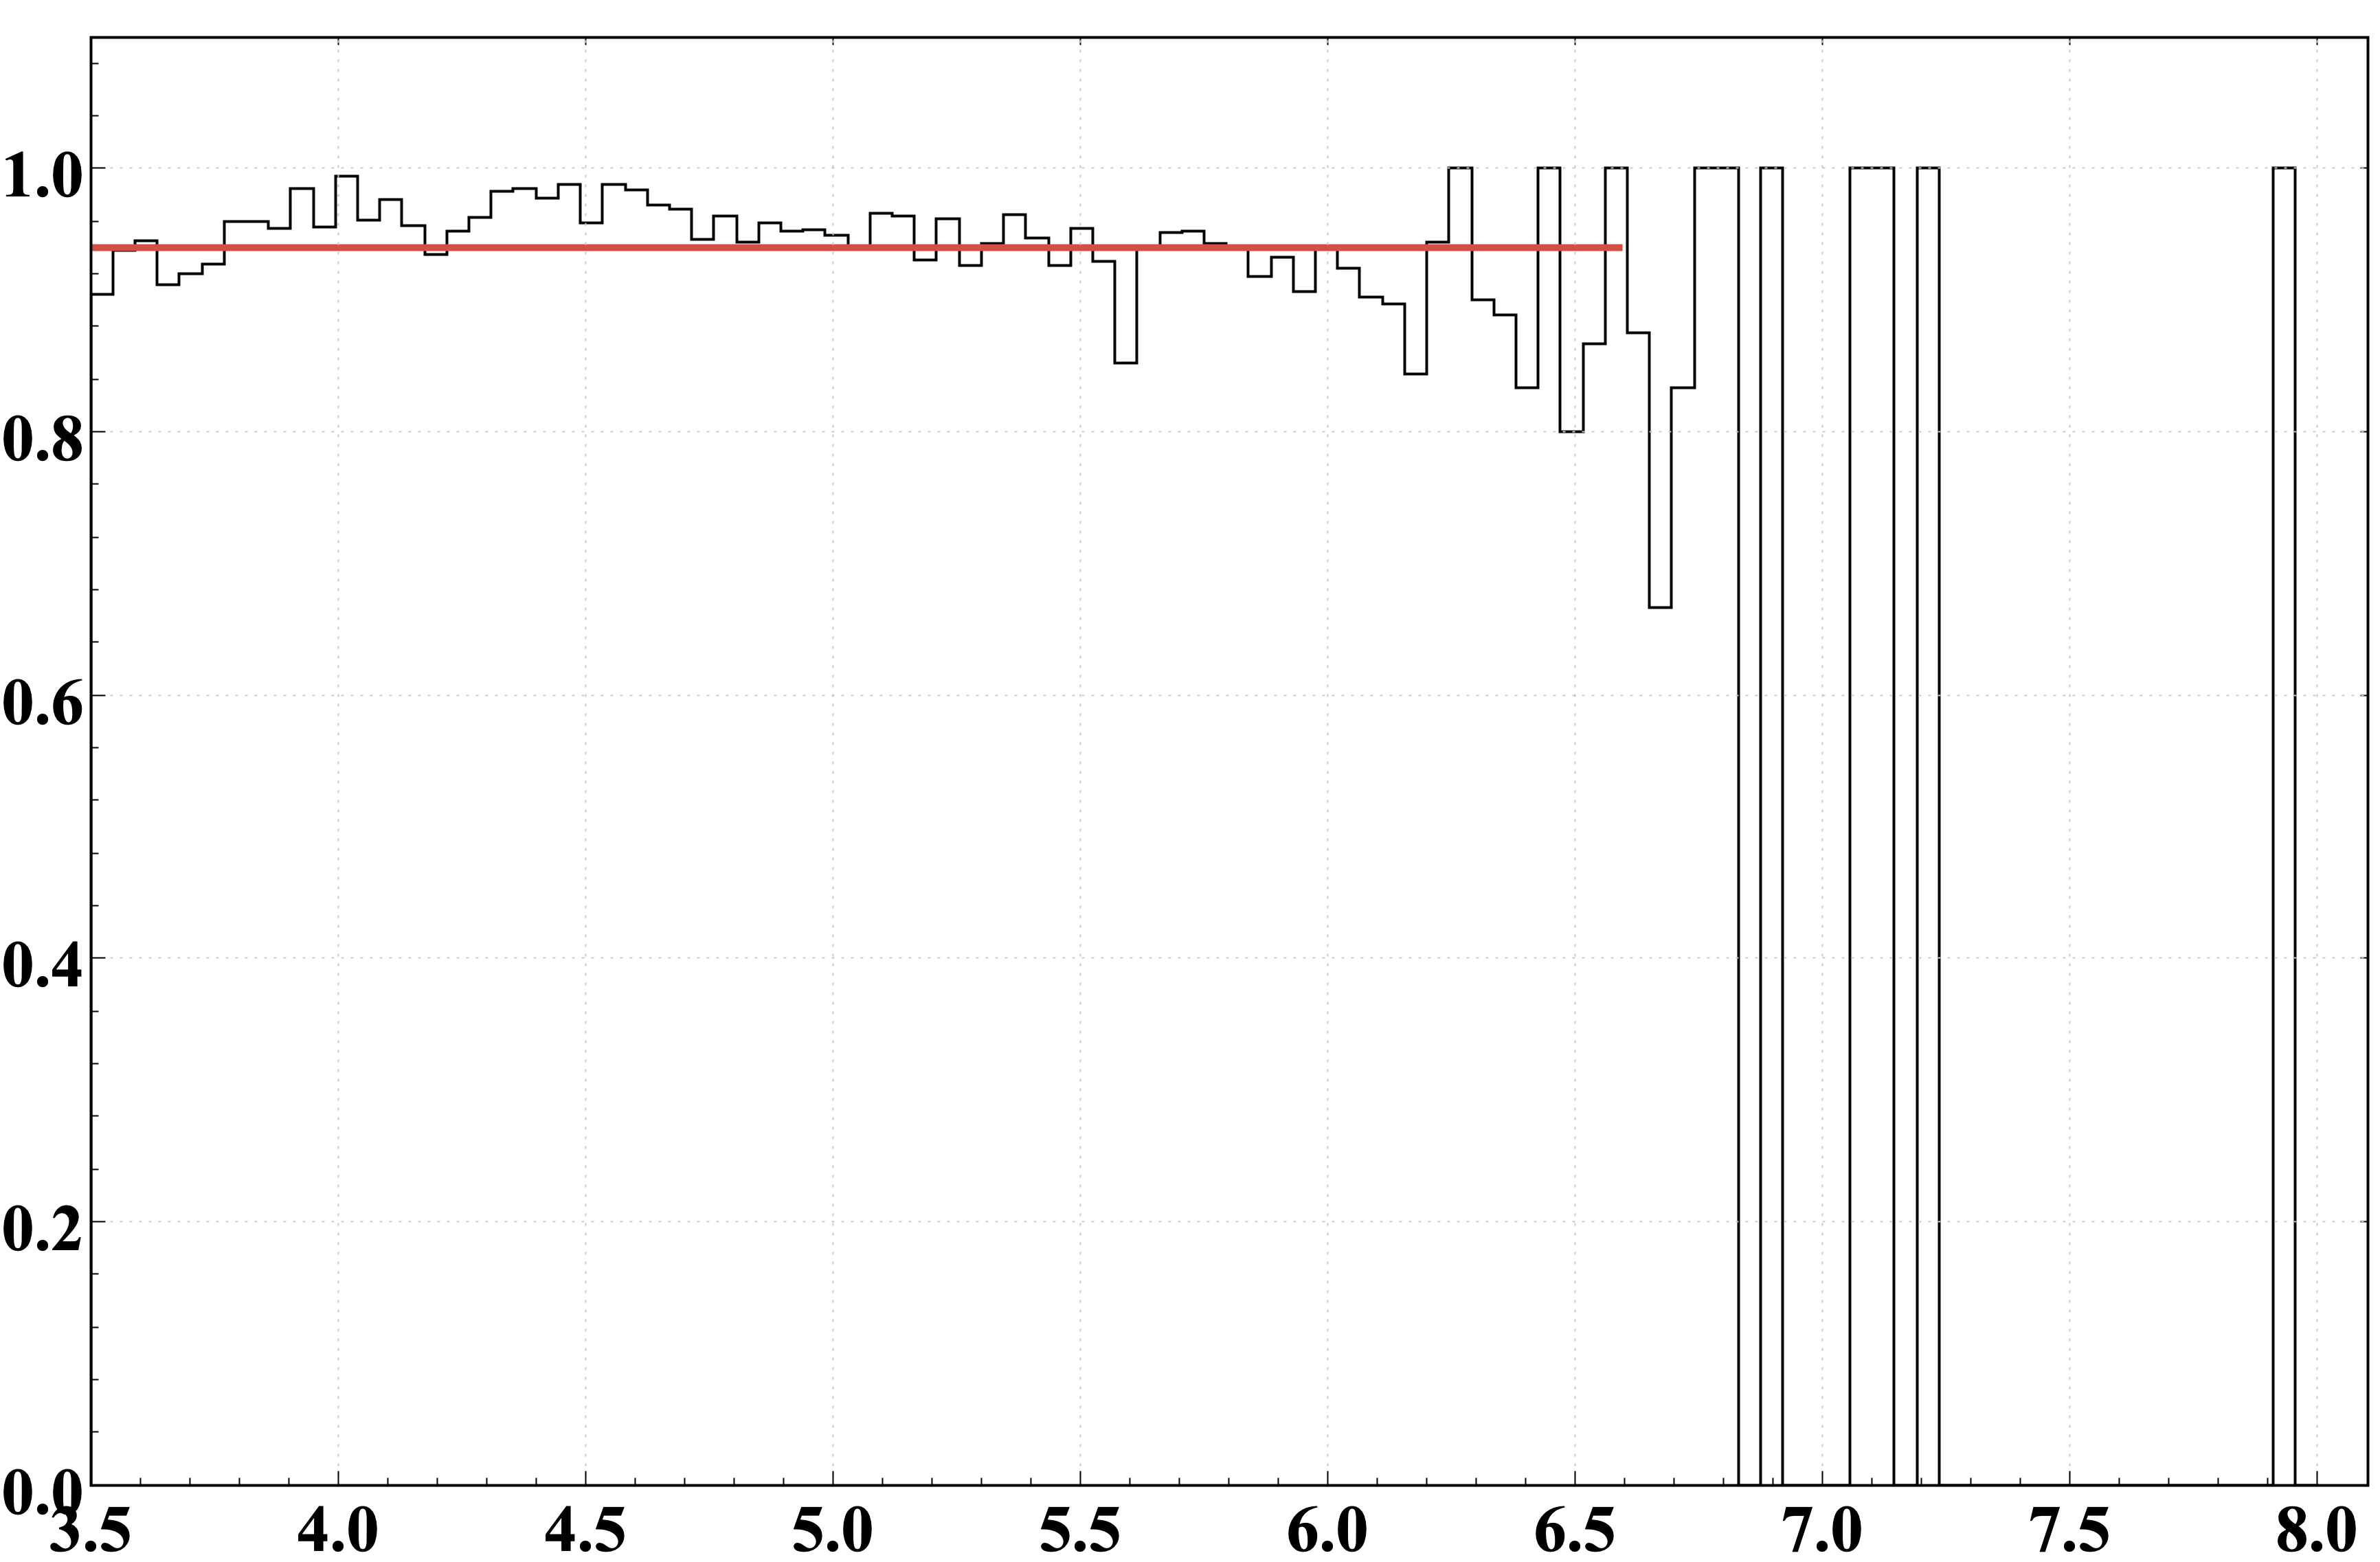
\includegraphics[width=0.98\columnwidth,keepaspectratio]{img/electronEfficiency.png}
	\caption{(placeholder) Top: the electron momentum spectrum before and after the requirement of an associated LTCC signal.
								  Bottom: the LTCC efficiency to electrons is the ration of the two distributions above.
								  A zero-order polynomial fit gives an average of 94$\%$ efficiency. }
	\label{fig:electronEfficiency}
\end{figure}

\subsection{LTCC Response to pions}

The calculate the response of the LTCC to pions, reconstructed positive pion particles are selected
and a check is done on whether they produced a signal in the LTCC detector or not.

The positive pions selection considers all the positvely charged particles that passed a neutron missing mass
cut relative to the reaction $eP\rightarrow e\pi^+N$.
The criterias for the event selections are:

\begin{itemize}
	\item  The electron selectio described in \ref{sec:elecResponse};
    \item Positive pion candidates $t^+$ are identified using the reconstruction event builder algorithm;
    \item The positive pion candidates must be within a detector fiducial cut, see \F{detFiducialCut}.
	\item The neutron missing mass $e^-t^+(n)$ is applied between 0.9 and 1.05 GeV (see \F{neutronMM}).
\end{itemize}

\begin{figure}
	\centering
	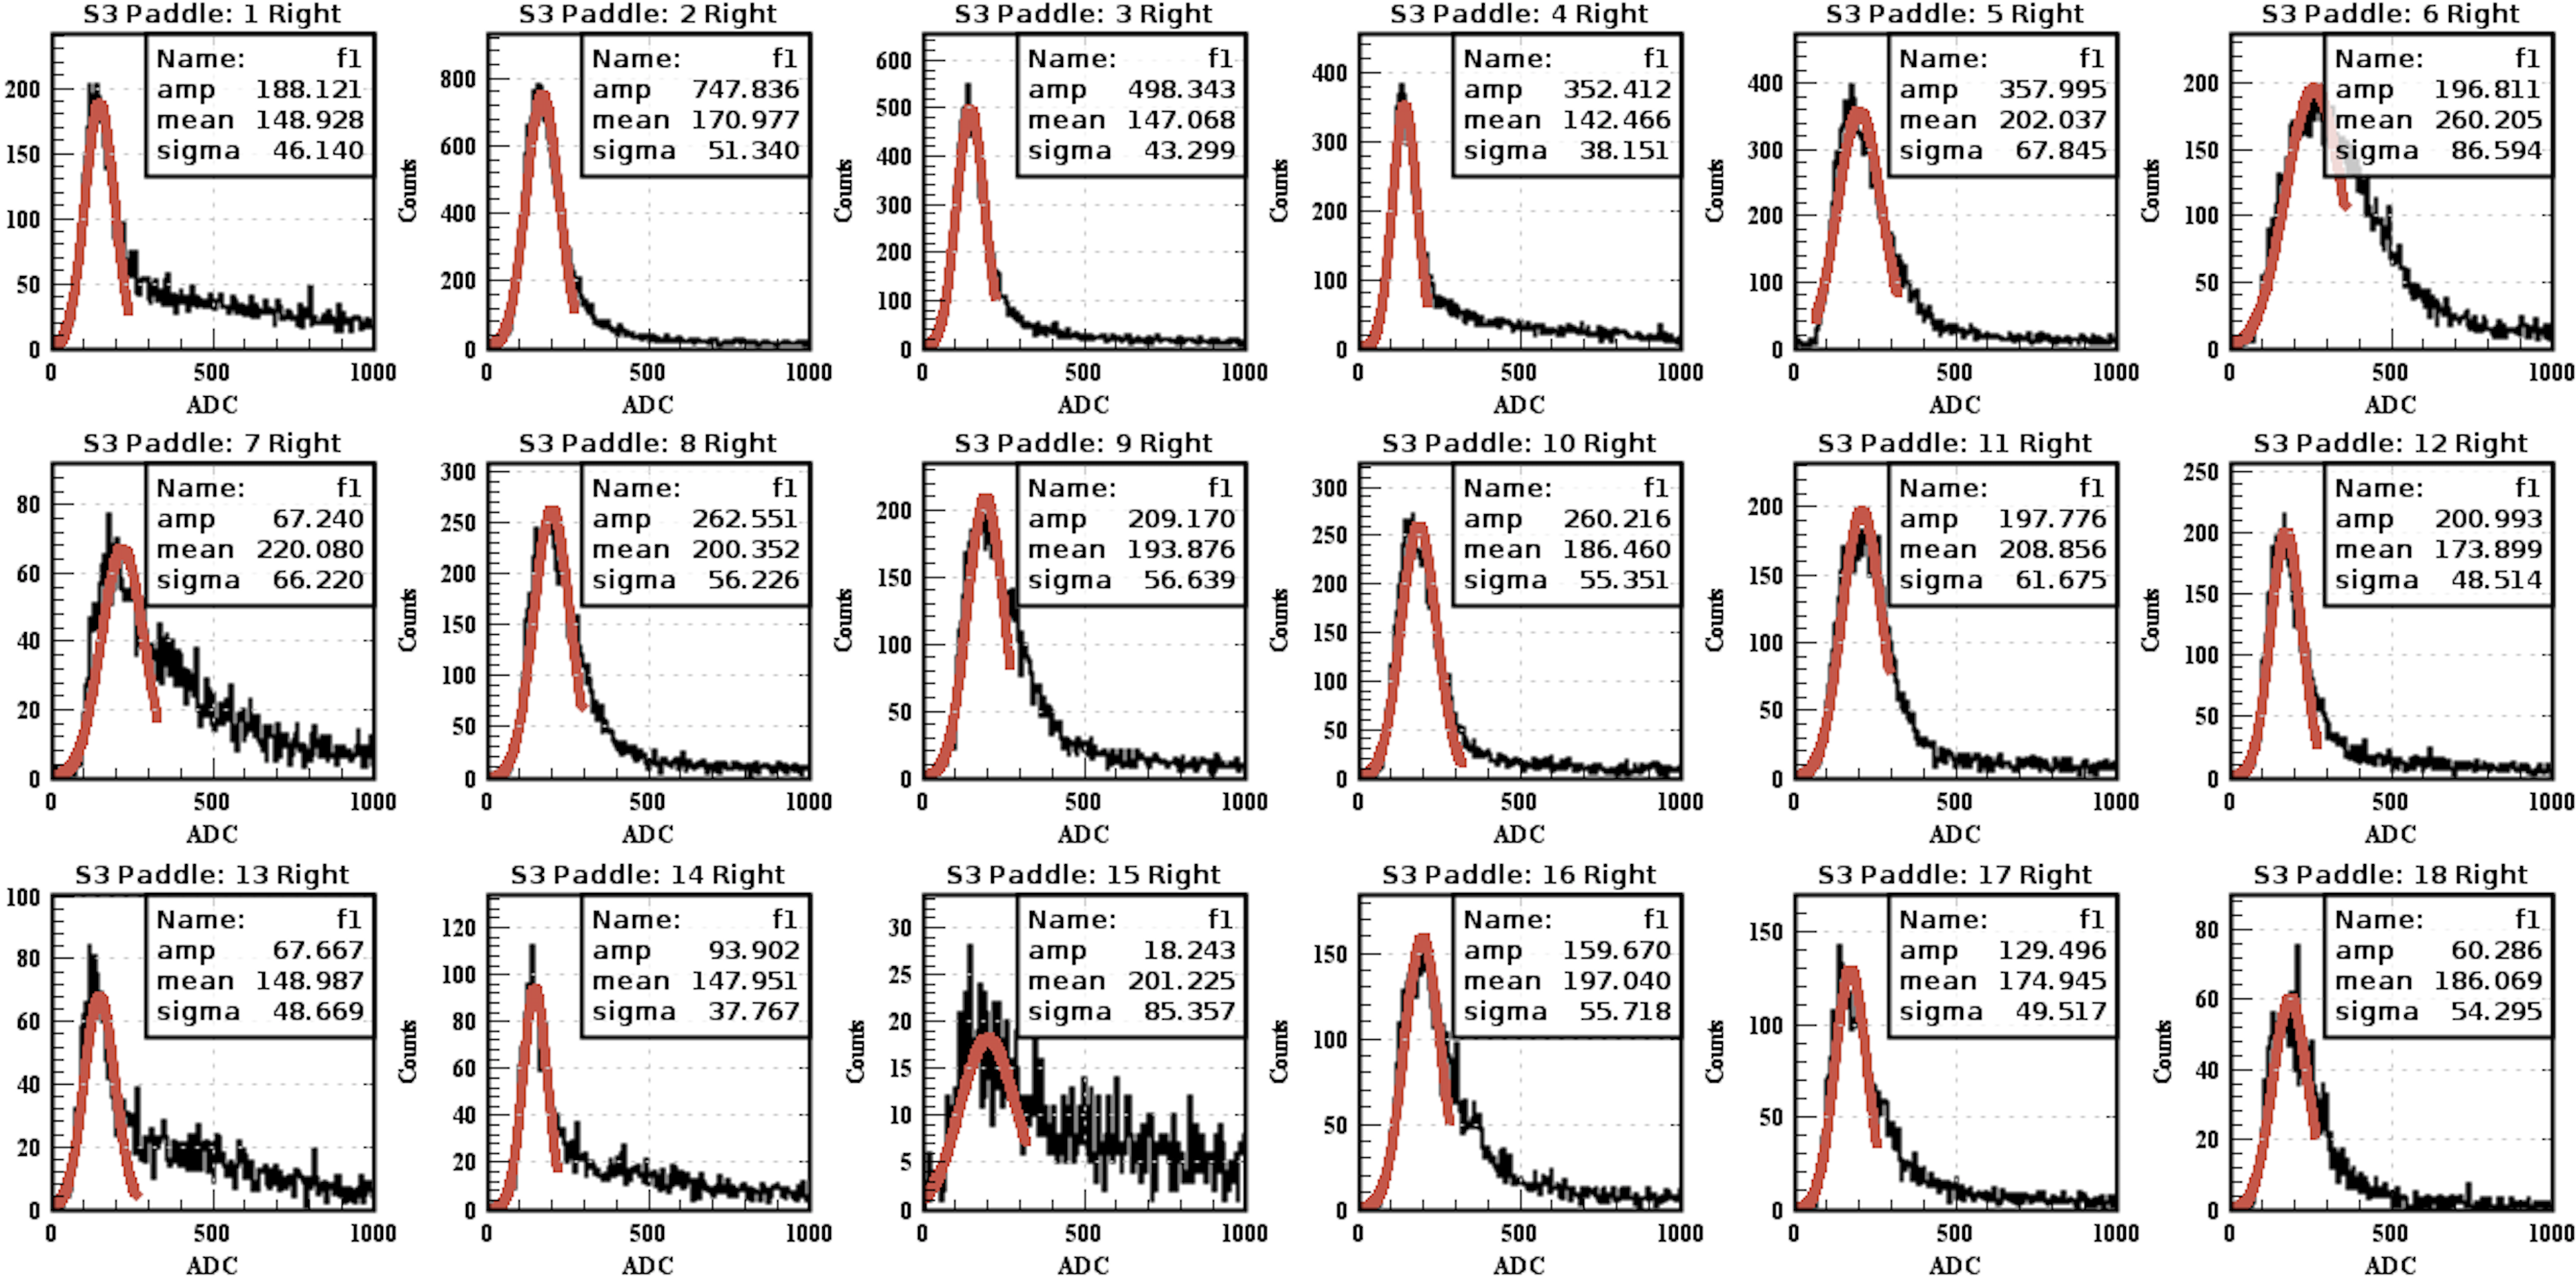
\includegraphics[width=0.98\columnwidth,keepaspectratio]{img/neutronMM.png}
	\caption{(placeholder) The fiducial cut applied to pions}
	\label{fig:detFiducialCut}
\end{figure}


The missing mass cut is shown in \F{neutronMM}. The positive pion candidates that satisfy the cuts are
labelled ``pions''.

\begin{figure}
	\centering
	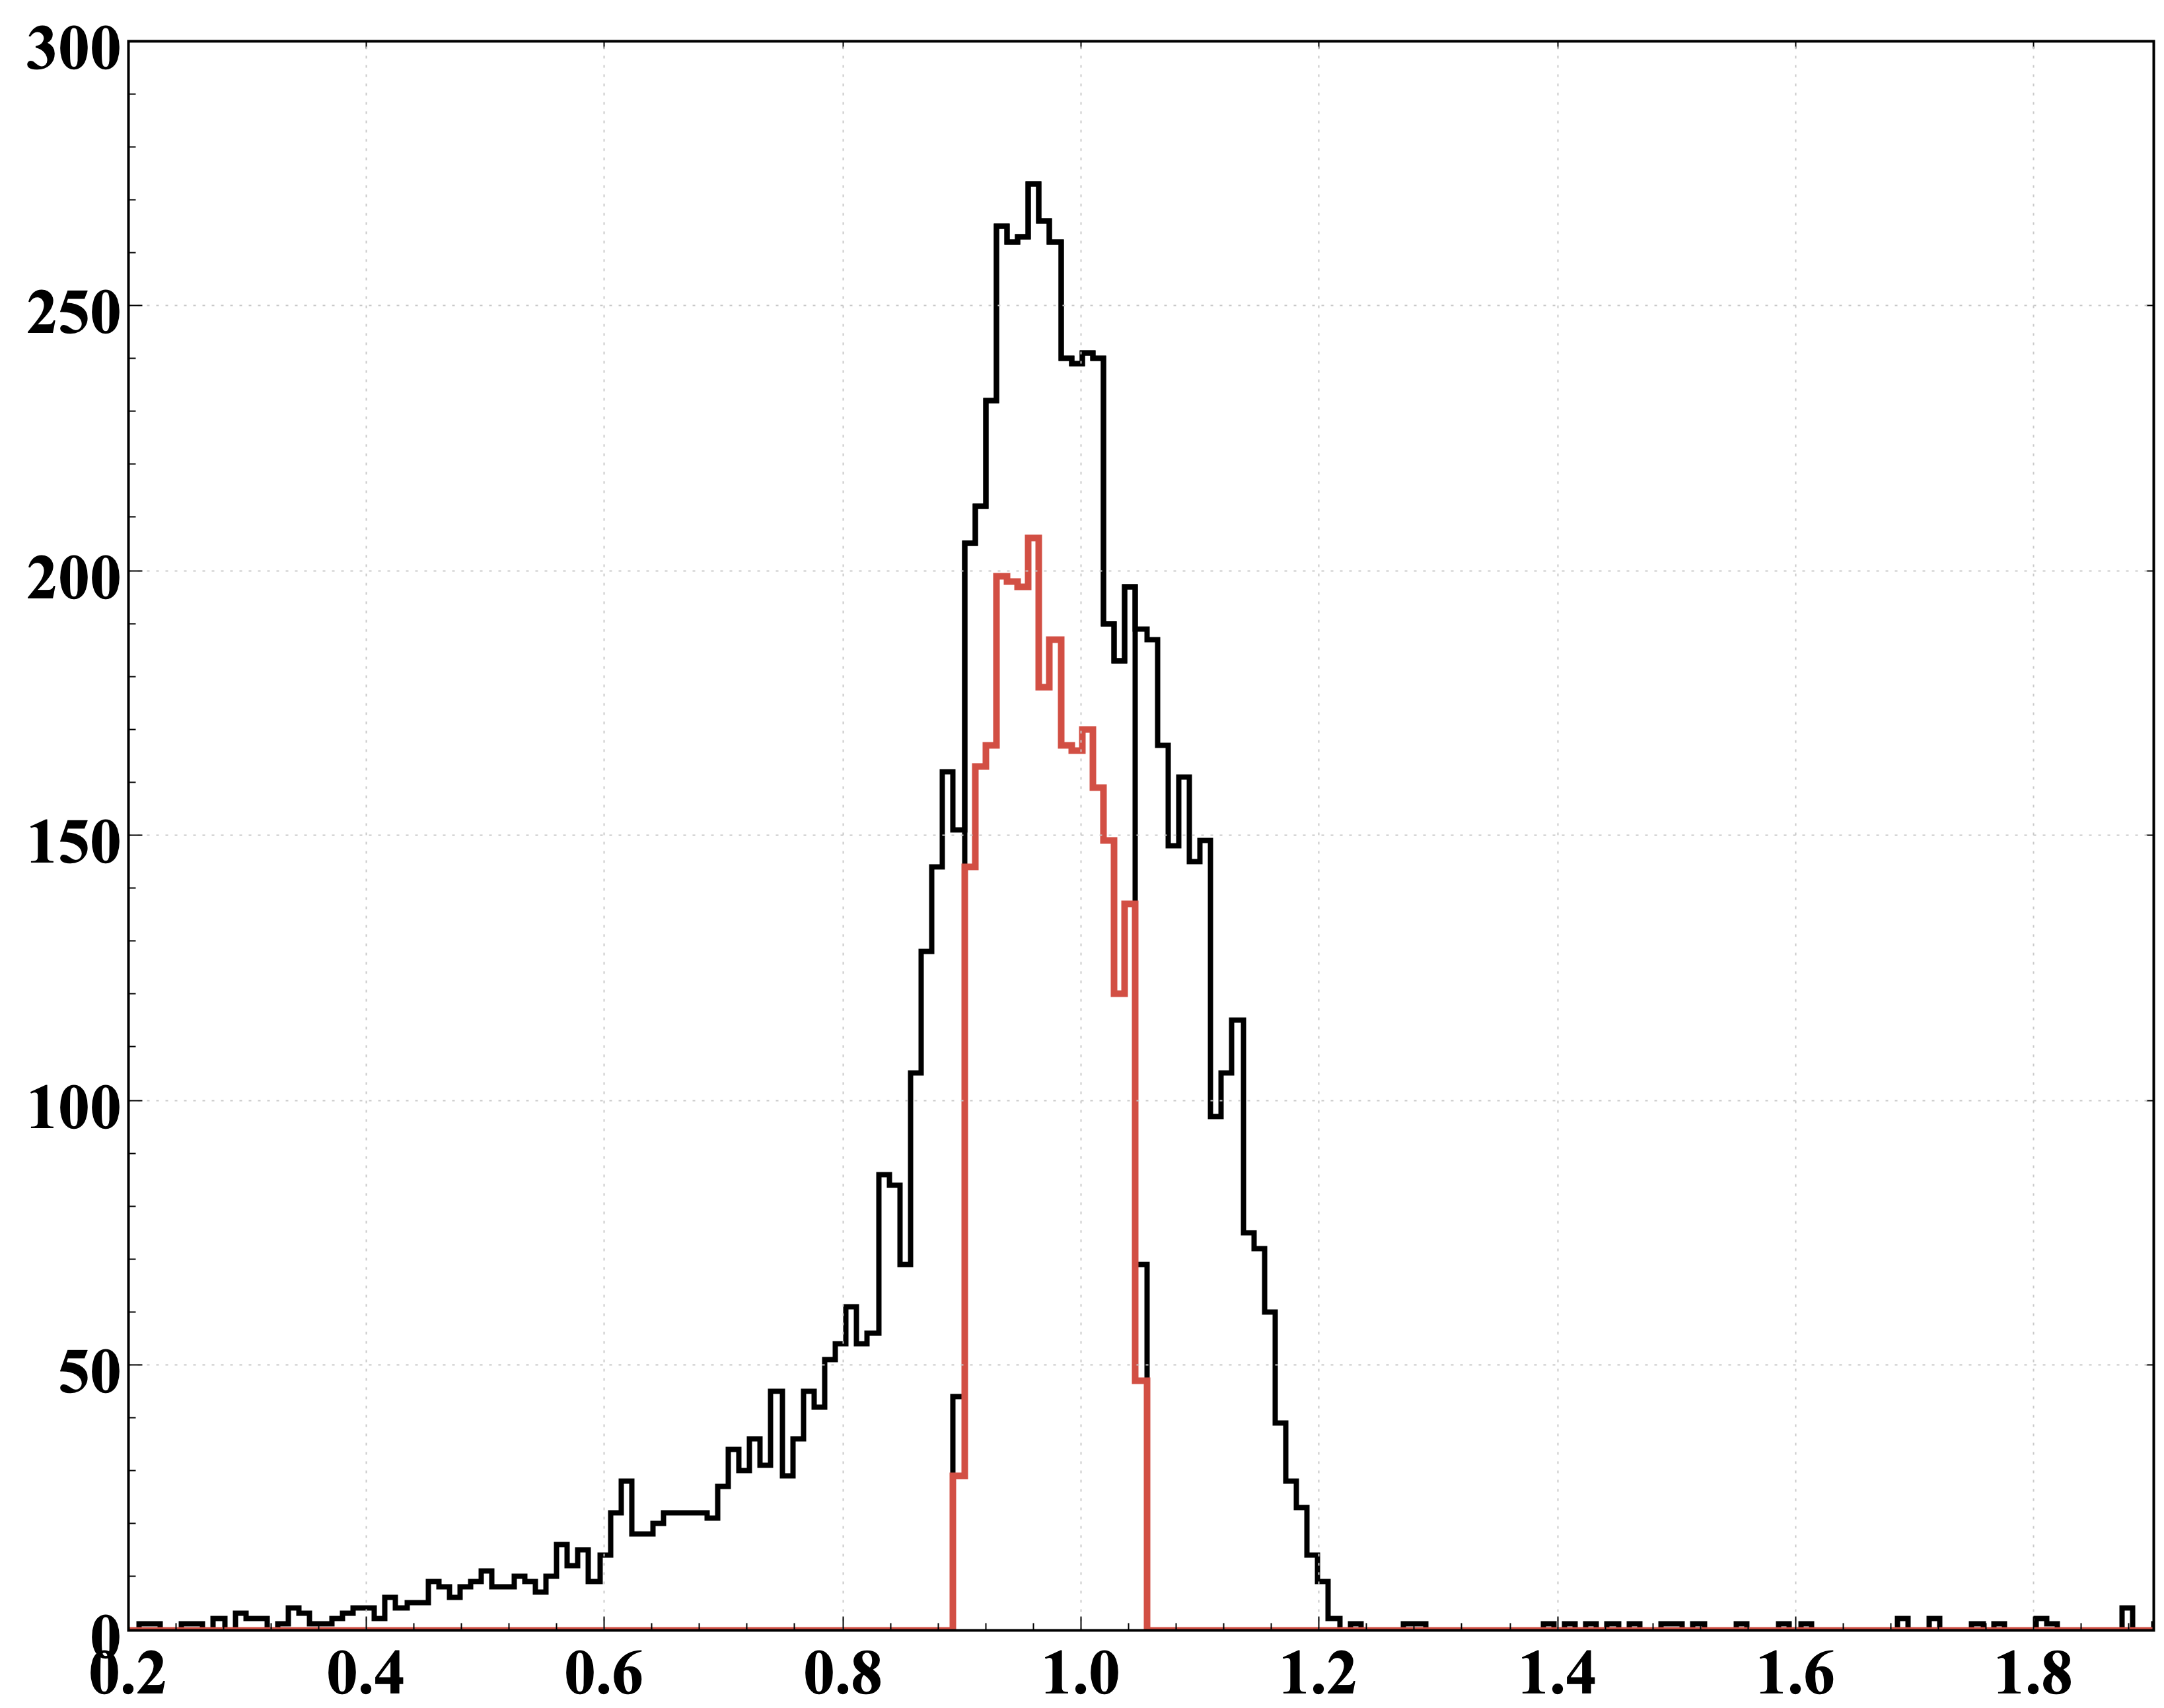
\includegraphics[width=0.98\columnwidth,keepaspectratio]{img/detFiducialCut.png}
	\caption{The neutron missing mass $mm = e^-t^+(n)$. The cuts are: 0.95 $<$ mm $<$ 1.05.
	         The positive pion candidates that satisfy the cuts are labelled “pions”.
				The pions associated with an LTCC signal are shown in red.}
	\label{fig:neutronMM}
\end{figure}

The momentum distribution of the pions is shown in \F{pionMomentum} for the all pions and for the pions
with an associated signal in the LTCC. The ratio


\begin{figure}
	\centering
	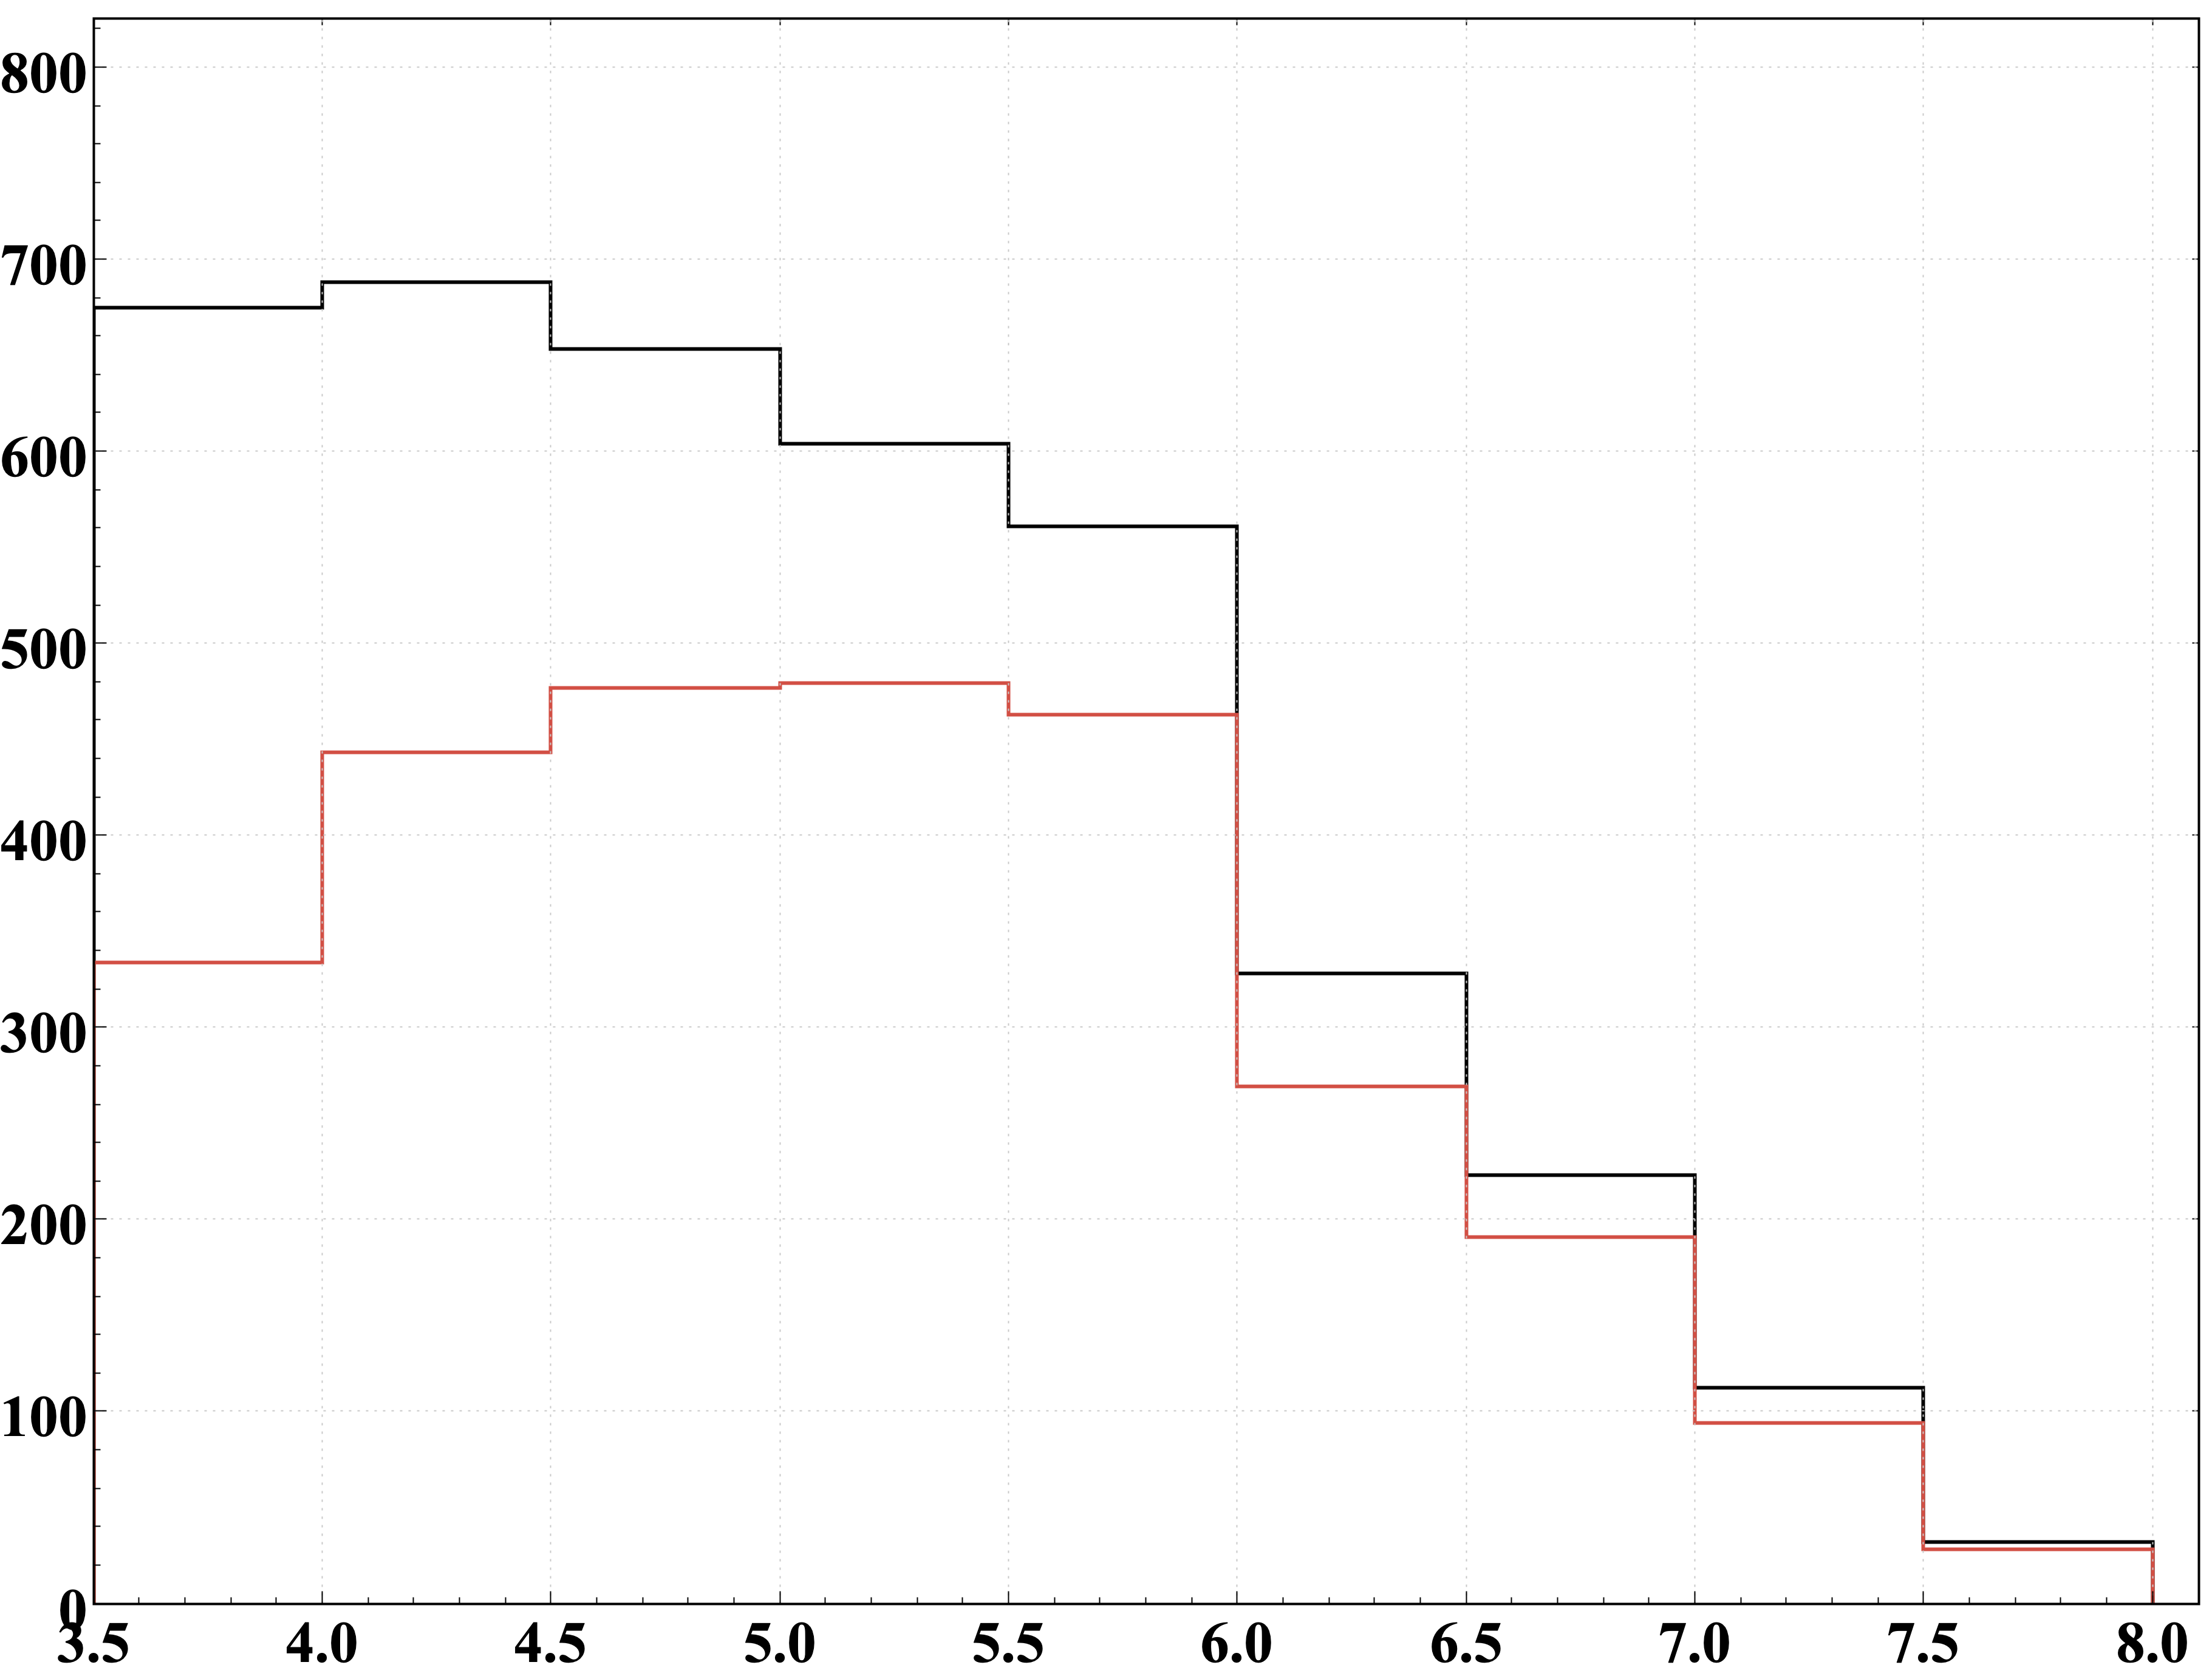
\includegraphics[width=0.98\columnwidth,keepaspectratio]{img/pionMomentum.png}
	\caption{The pion momentum distribution before and after the requirement of an associated LTCC signal. }
	\label{fig:pionMomentum}
\end{figure}


The pions efficiency, shown in \F{pionEfficiency}, is normalized to the electrons to account for the detector
inefficiencies unrelated to the LTCC. The LTCC response starts around 50$\%$ near the expected signal threshold,
and rise with momentum as expected. A plateau of 85$\%$ is reached after a momentum of 5 GeV / c.
This is within range of an expectation of efficiency above 90$\%$. Among the possible reasons for this shortcoming:

\begin{itemize}
	\item   the optical alignment of the mirrors, which was a compromise between
	        positive and negative charged tracks instead of optimizing it for negative tracks only;
    \item  the  $C_4F_{10}$ gas used in the spring 2019 experiment did not go through a purification cycle and
			  may have contained some impurities.
\end{itemize}


\begin{figure}
	\centering
	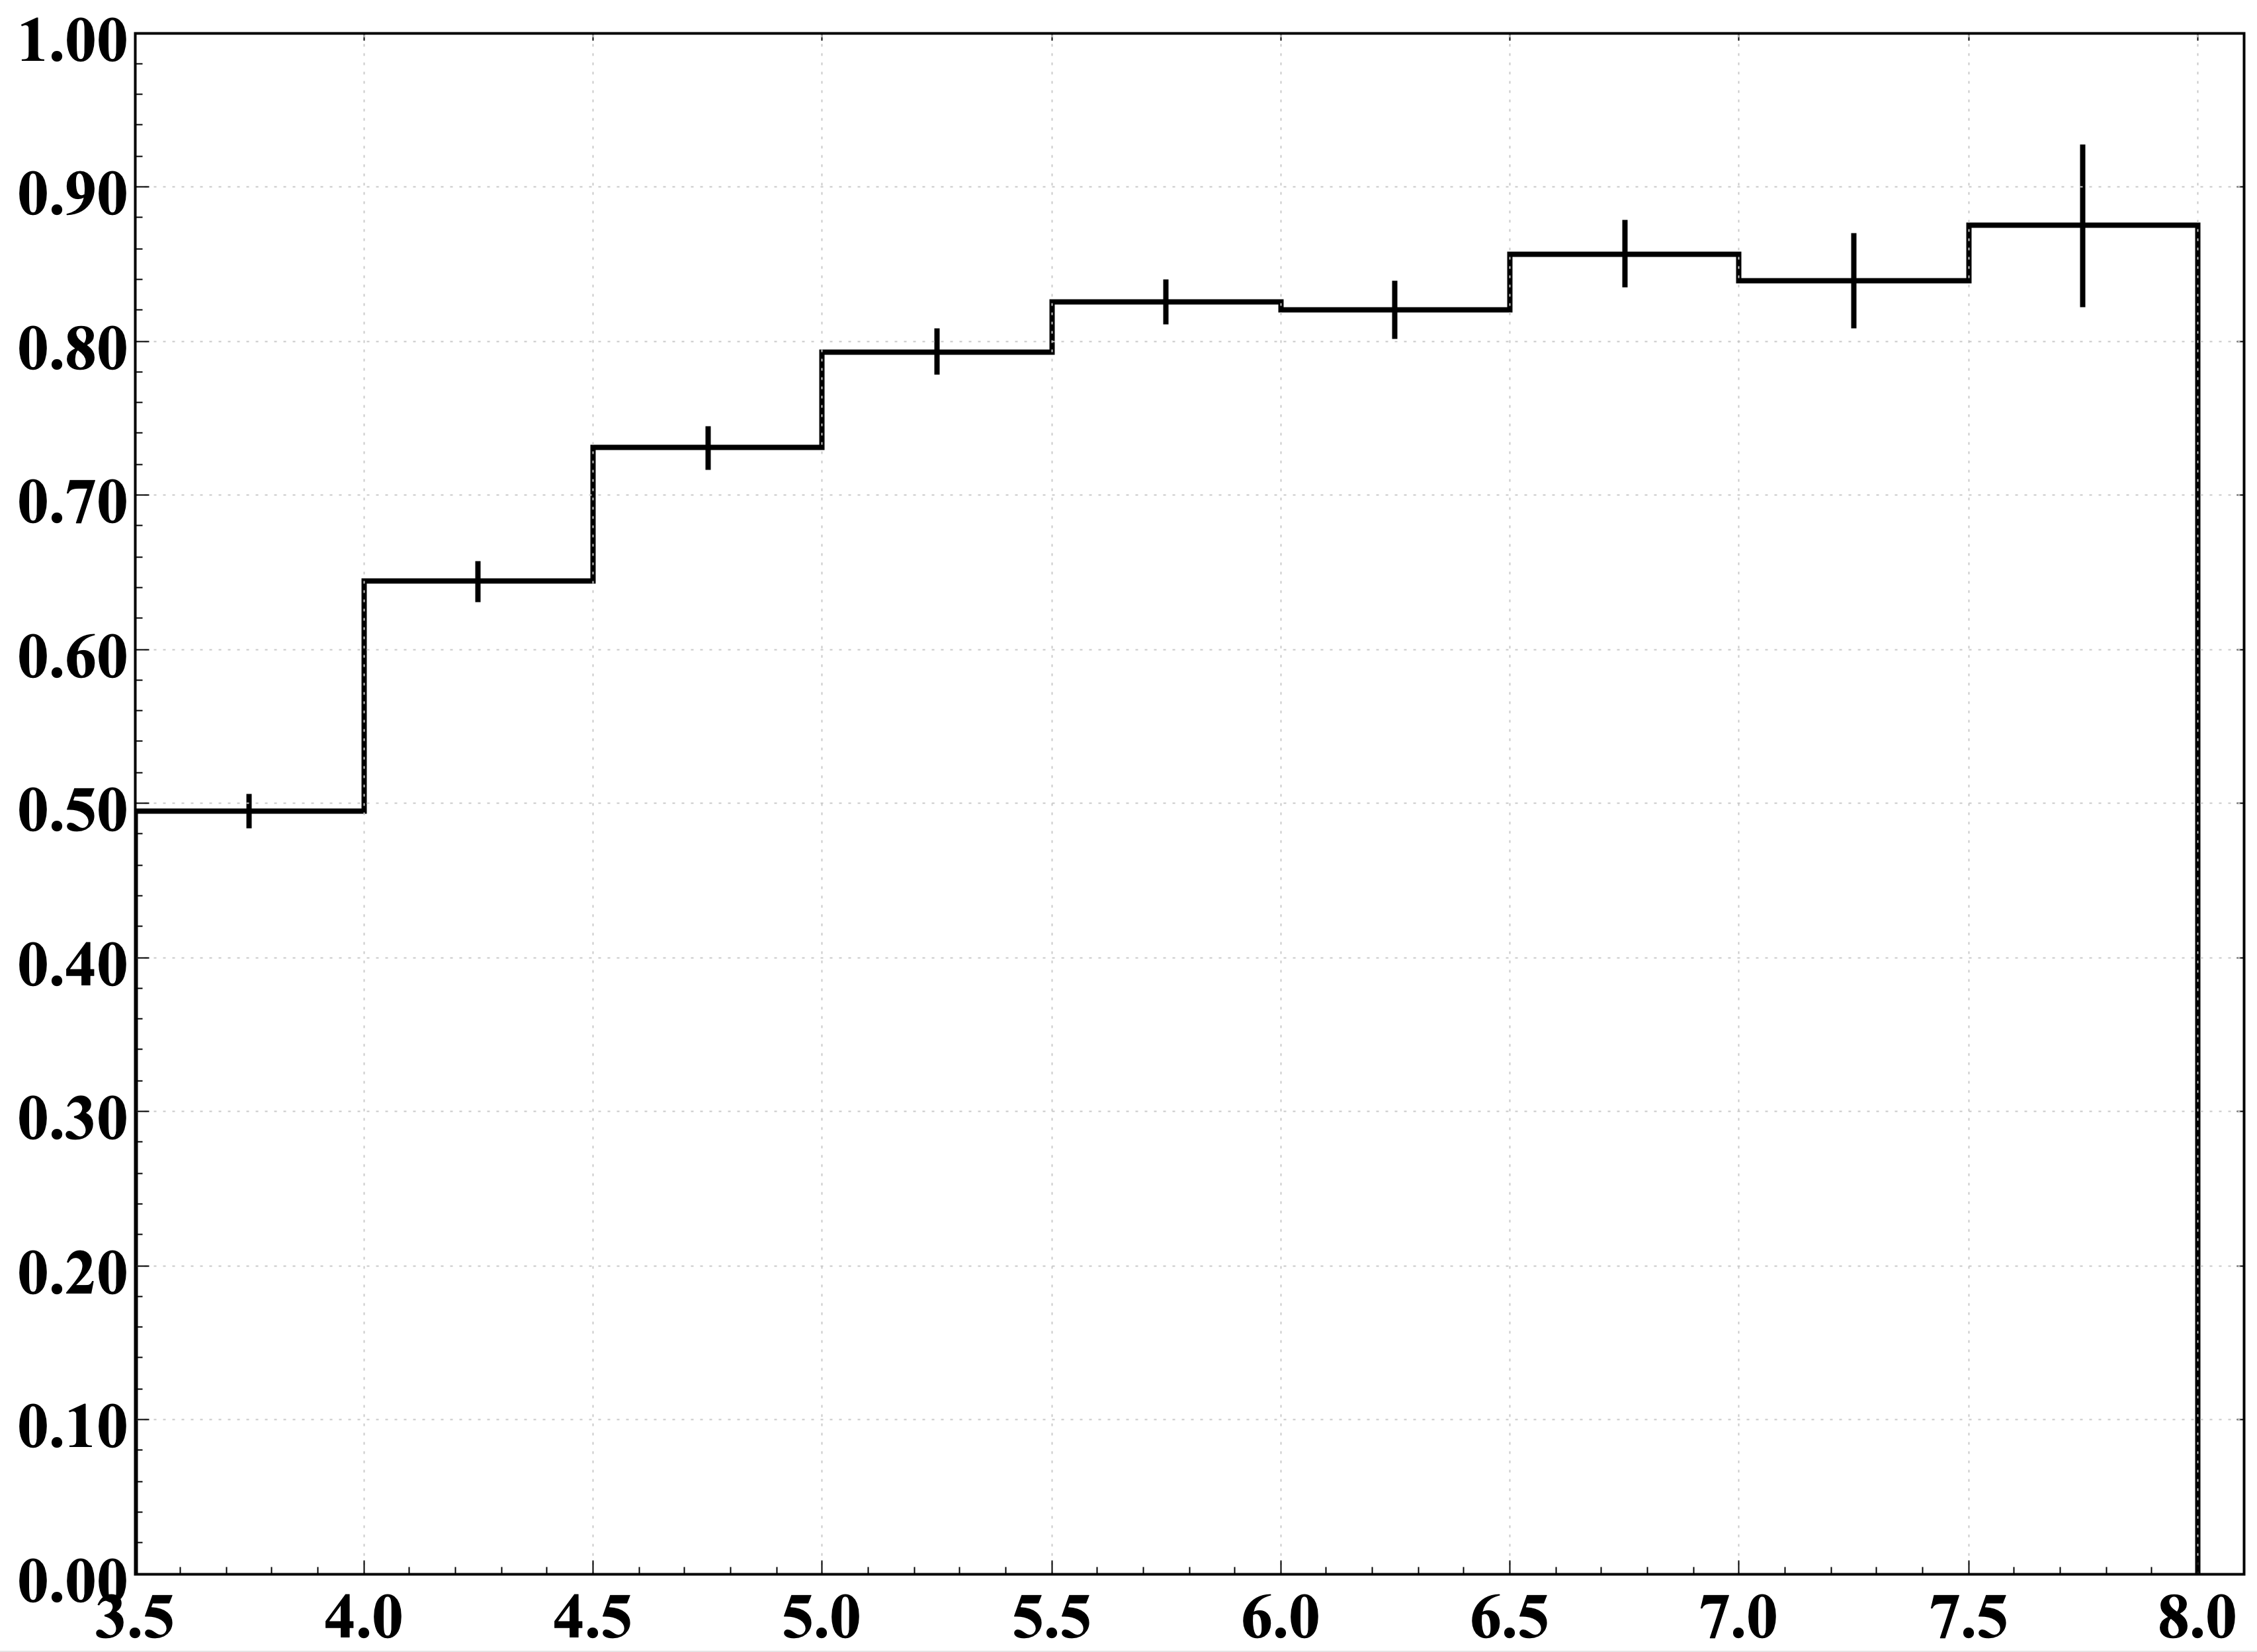
\includegraphics[width=0.98\columnwidth,keepaspectratio]{img/pionEfficiency.png}
	\caption{(placeholder: not normalized to electron yet) The LTCC pion efficiency as a function of momentum.  }
	\label{fig:pionEfficiency}
\end{figure}






